%% This is an example first chapter.  You should put chapter/appendix that you
%% write into a separate file, and add a line \include{yourfilename} to
%% main.tex, where `yourfilename.tex' is the name of the chapter/appendix file.
%% You can process specific files by typing their names in at the 
%% \files=
%% prompt when you run the file main.tex through LaTeX.
% \newtheorem{example}{Example}
\newtheorem{definition}{Definition}

\newcommand{\dt}{h}
\newcommand{\qu}{{q^\mathrm{u}}}
\newcommand{\qa}{{q^\mathrm{a}}}
\newcommand{\qacmd}{{q^\mathrm{a}_\mathrm{cmd}}}
\newcommand{\dqu}{{\delta q^\mathrm{u}}}
\newcommand{\dqa}{{\delta q^\mathrm{a}}}
\newcommand{\dq}{{\delta q}}
\newcommand{\Ka}{\mathbf{K}_\mathrm{a}}
\newcommand{\ka}{k_\mathrm{a}}
\newcommand{\Mu}{\mathbf{M}_\mathrm{u}}
\newcommand{\Ba}{\mathbf{B}^\mathrm{a}}
\newcommand{\Bu}{\mathbf{B}^\mathrm{u}}
\newcommand{\BuBundle}{\mathbf{\hat{B}}_\mathrm{u}}
\newcommand{\tauU}{\tau^\mathrm{u}}
\newcommand{\tauA}{\tau^\mathrm{a}}
\newcommand{\J}{\mathbf{J}}
\newcommand{\Ju}[1][]{\mathbf{J}_{\mathrm{u}_{#1}}}
\newcommand{\Ja}[1][]{\mathbf{J}_{\mathrm{a}_{#1}}}
\newcommand{\Jn}[1][]{\mathbf{J}_{\mathrm{n}_{#1}}}
\newcommand{\Jt}[1][]{\mathbf{J}_{\mathrm{t}_{#1}}}
\newcommand{\JuActive}{\tilde{\mathbf{J}}_\mathrm{u}}
\newcommand{\JaActive}{\tilde{\mathbf{J}}_\mathrm{a}}
\newcommand{\R}[1][]{\mathbb{R}^{#1}}
\newcommand{\nU}{n_\mathrm{u}}
\newcommand{\nA}{n_\mathrm{a}}
\newcommand{\nC}{n_\mathrm{c}}
\newcommand{\nCG}{n_\mathrm{cg}}
\newcommand{\RbarU}[1]{\bar{\mathcal{R}}^\mathrm{u}_{#1}}
\newcommand{\norm}[1]{\left\lVert{#1}\right\rVert}
\newcommand{\SigmaInverse}{\hat{\mathbf{\Sigma}}^{-1}}
\newcommand{\distanceU}{\hat{d}^\mathrm{u}}
\newcommand{\qNominalU}{\bar{q}^\mathrm{u}}
\newcommand{\qNominalA}{\bar{q}^\mathrm{a}}
\newcommand{\qNominalACmd}{\bar{q}^\mathrm{a}_\mathrm{cmd}}
\newcommand{\muHatU}{\hat{\mu}^\mathrm{u}}
\newcommand{\xgoal}{x_\text{goal}}
\newcommand{\minimize}{\mathrm{min}.}
\newcommand{\DfDx}[2]{\frac{\partial {#1}}{\partial {#2}}}
\newcommand{\DfDxLine}[2]{\partial {#1} / \partial {#2}}
\newcommand{\A}{\mathbf{A}}
\newcommand{\B}{\mathbf{B}}
\newcommand{\I}{\mathbf{I}}
\newcommand{\code}[1]{{\fontfamily{cmss}\selectfont {#1}}}

\newcommand{\Nearest}{\mathtt{Nearest}}
\newcommand{\Extend}{\mathtt{Extend}}
\newcommand{\ContactSample}{\mathtt{ContactSample}}

% aliases
\newcommand{\mb}[1]{\mathbf{#1}}


% Control
\newcommand{\qcmd}[1][]{q_{\text{cmd}}^{#1}}
\newcommand{\qref}[1][]{q_{\text{ref}}^{#1}}
\newcommand{\tauE}{\tau_{\text{ext}}}
\newcommand{\tauM}{\tau_{\text{m}}}
\newcommand{\myul}[2]{\setulcolor{#1}\ul{#2}\setulcolor{black}}
\newcommand{\quantity}[4]{{}^{#2}{#1}^{#3}_{#4}} % 1: quantity name, 2: 'from' frame, 3: 'to' frame, 4: 'expressed-in' frame.
\newcommand{\transpose}[1]{\left({#1}\right)^\intercal}

% Sensing
\newcommand{\numcontact}{N} % number of contacts
\newcommand{\contacts}{P} % collection of contacts
\newcommand{\contact}[1]{p^{#1}} % contact location
\newcommand{\deltaq}{\delta_{q}} % change in pose
\newcommand{\real}{\mathbb{R}}
\newcommand{\numjoints}{{n_q}} % number of joints in robot
\newcommand{\pull}{b}  % pull binary
\newcommand{\binary}{\{0, 1\}} 
\newcommand{\ones}{\mathbf{1}} 
\newcommand{\transp}{^\intercal} 
\newcommand{\normal}[1]{n_i} % surface normal
\newcommand{\jackobian}[1]{\mathbf{J}_i} % Jacobian
\newcommand{\minpull}{\epsilon_\text{pull}^\text{min}}
\newcommand{\maxpull}{\epsilon_\text{pull}^\text{max}}
\newcommand{\minpush}{\epsilon_\text{push}^\text{min}}
\newcommand{\maxpush}{\epsilon_\text{push}^\text{max}}
\newcommand{\maxrad}{{r_\text{orth}}}
\newcommand{\dqmax}{\deltaq^\text{max}}
\newcommand{\dpos}{\delta p} % change in pose

\newcommand{\pCbar}{p_{C}}
\newcommand{\pC}{{p}_C}
\newcommand{\fC}{{f}_C}


\chapter{Introduction}
In 1988, Salisbury et al. from the MIT AI lab envisioned \emph{contact-rich} robotic manipulators that ``employ all the available manipulation surfaces of the robot to \emph{act} upon and \emph{sense} the environment'', in a way similar to how humans interact with the environment using their limbs and torso \cite{salisbury1988preliminary}. This was in stark contrast with the prevailing practice in robotic manipulation back then, where environmental interaction is limited ``at the hand of the arm'', while the arm itself needs to carefully avoid contacts. Unfortunately, real-world deployment of contact-rich robotic manipulators still remains elusive even after more than 30 years. In most contemporary commercial applications of robotic manipulation, such as in warehouses or on factory floors, the robotic manipulator is still divided into the touching hand and the collision-avoiding arm \cite{beautifulamazon}. 
The dichotomy between the hand and the arm is also prominent in robotics research: although increasingly effective algorithms for grasping objects with the hand \cite[\textsection 17]{siciliano2008springer} and avoiding obstacles with the arm \cite{lavalle1998rapidly, marcucci2022motion} have been developed over the decades, a reliable, generalizable and interpretable solution to human-like contact-rich manipulation still remains to be found. 

\section{Difficulty of Pushing a Box with a Ball \label{sec:intro:box_ball_system}}
The difficulty of contact-rich manipulation planning is rooted in the non-smooth nature of contact dynamics. In this section, we hope to illustrate this difficulty using a simple task that involves just one contact: pushing a box with a ball in 1D (1-Dimension). 
As shown in Fig. \ref{fig:intro:1d_box_ball}, the system consists of an \emph{un-actuated} box which slides along a rail with sufficient damping, and an \emph{actuated} ball controlled by a Proportional-Derivative (PD) controller. 
The position of the box is denoted by $\qu \in \mathbb{R}$. The actual and commanded positions of the ball are denoted respectively by $\qa \in \mathbb{R}$ and $u \in \mathbb{R}$. 
The ball can push on the left (Fig. \ref{fig:intro:1d_box_ball}a) or right (Fig. \ref{fig:intro:1d_box_ball}b) surface of the box.

\begin{figure}[t]
\centering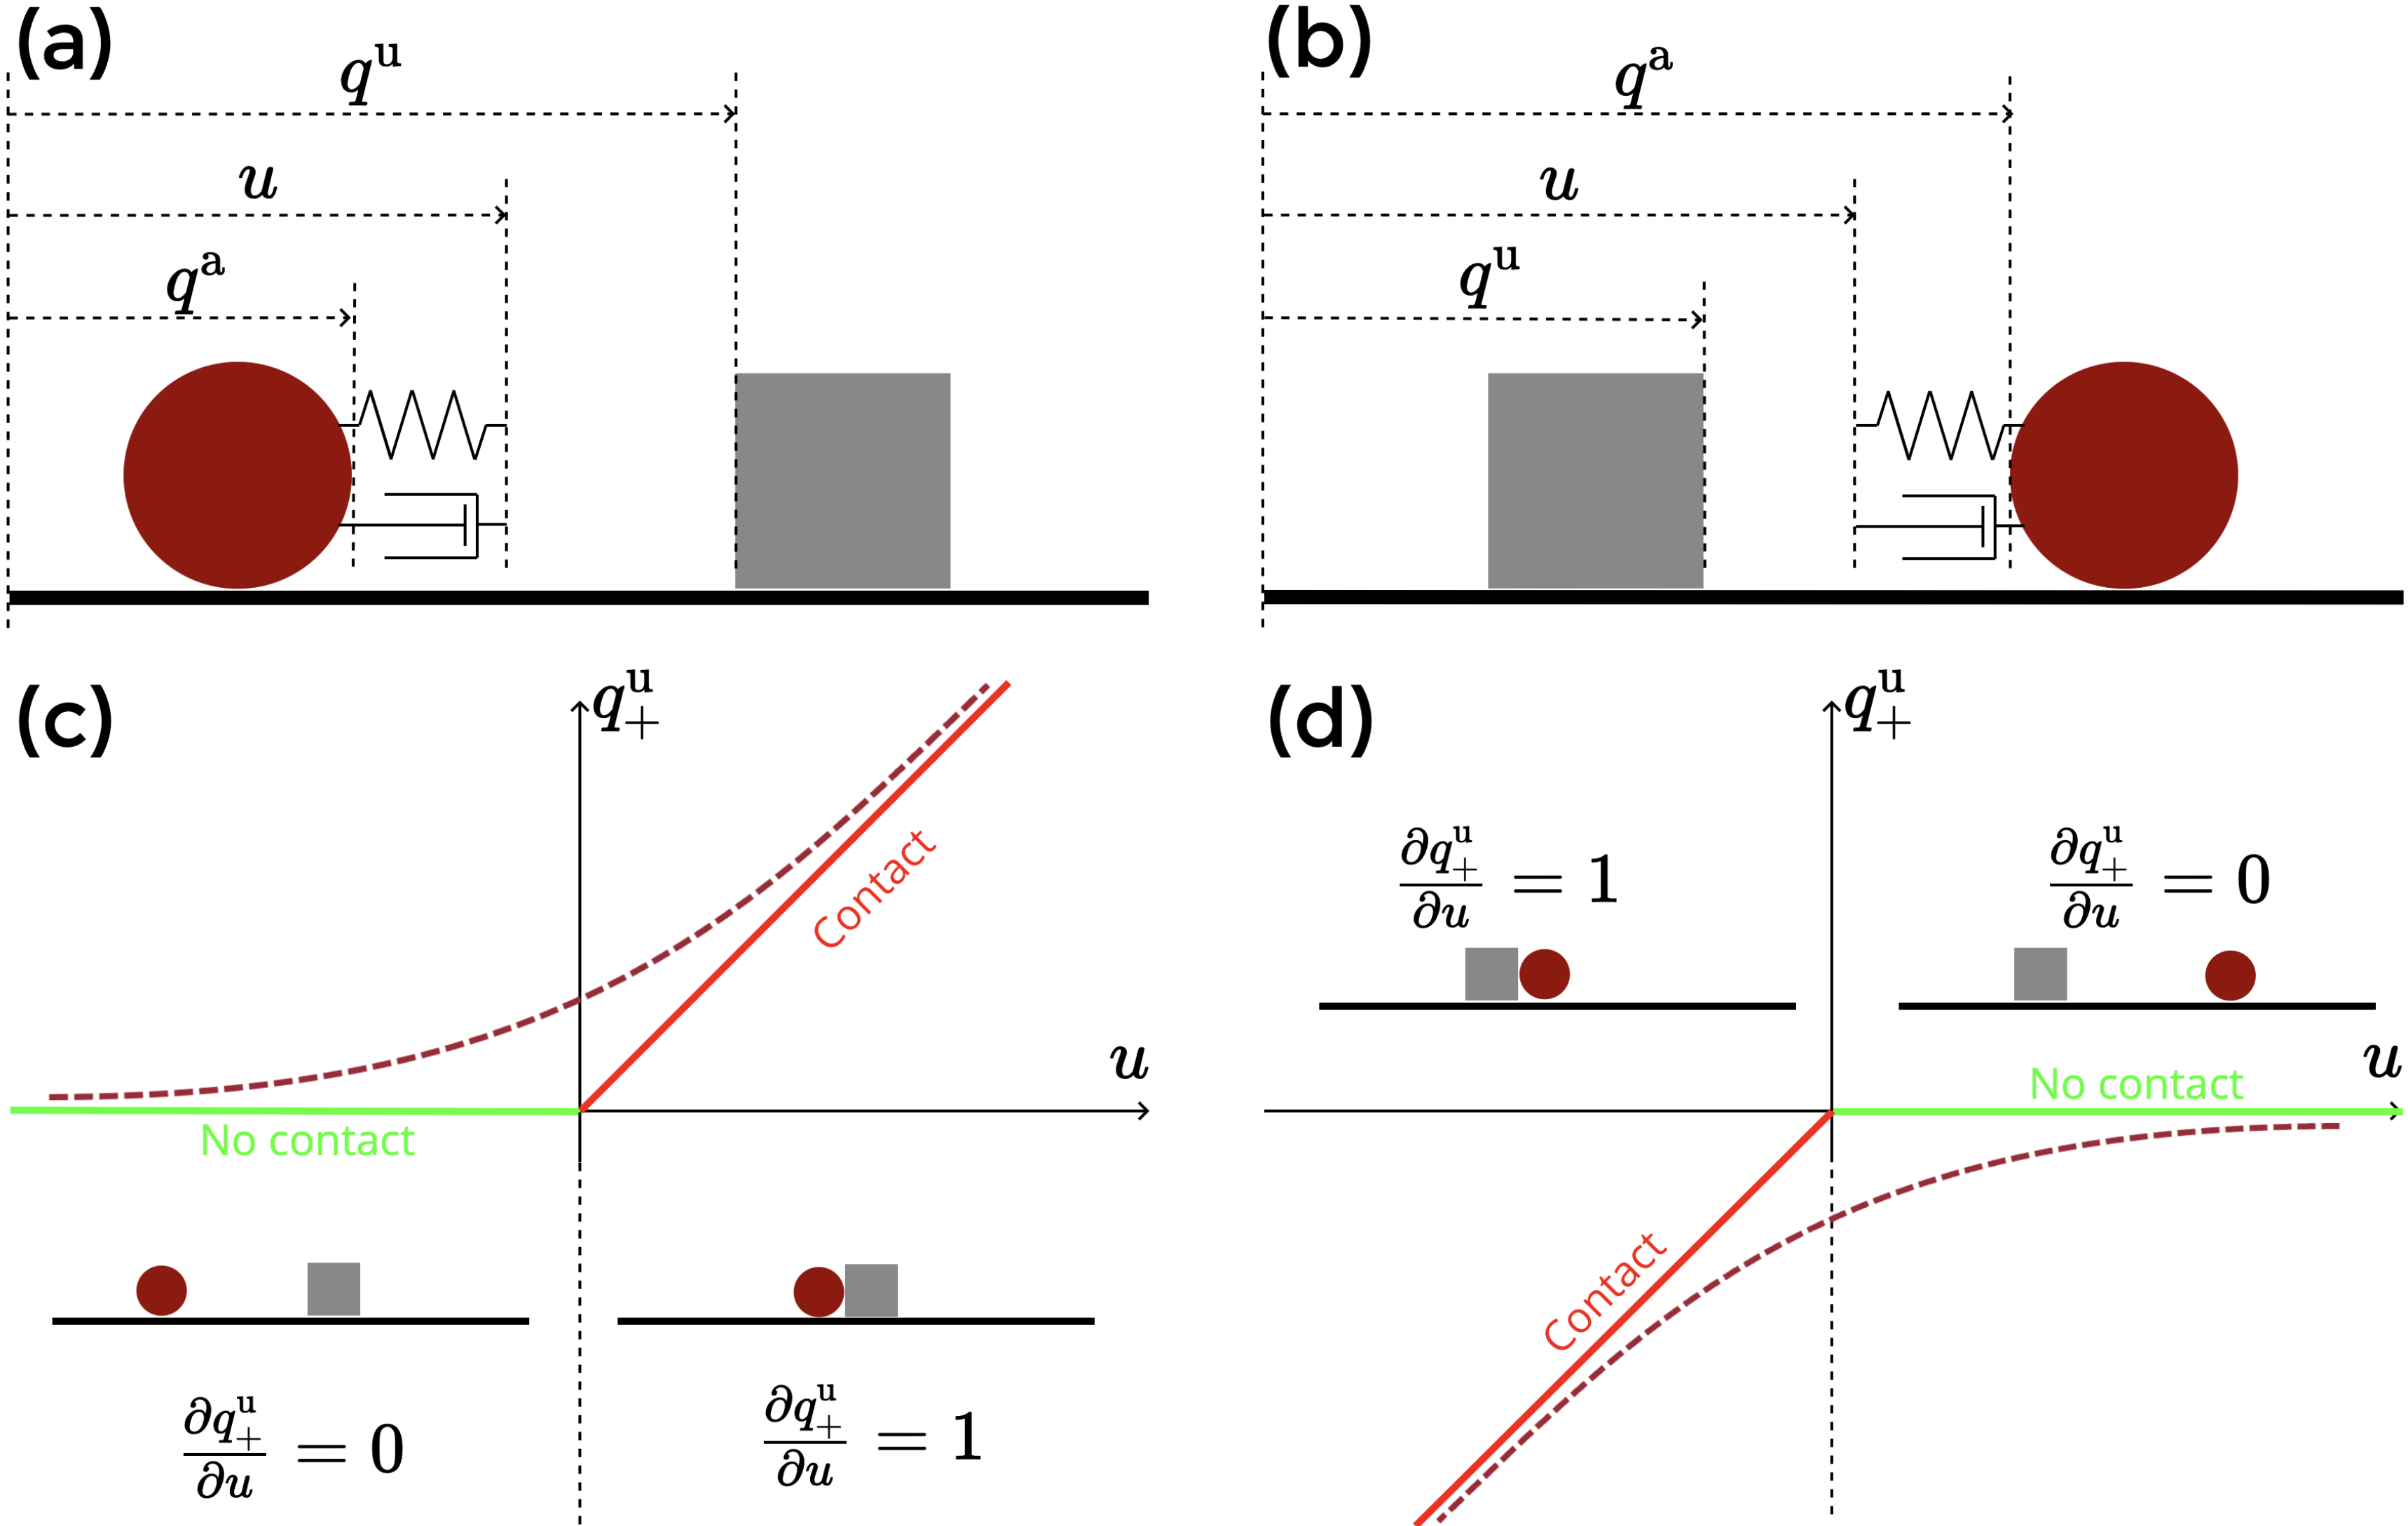
\includegraphics[width = 0.95\textwidth]{figures/01_intro/1d_box_ball.png}
\caption{(\textbf{a-b}) An actuated, PD-controlled ball and an un-actuated box, both are constrained to slide along a rail. (\textbf{a}): Ball on the left of the box. (\textbf{b}): Ball on the right of the box. (\textbf{c-d}) Dynamics of the ball-box system when the ball is on the (\textbf{c}) left or (\textbf{d}) right side of the box. Red and green indicate different contact modes. The maroon dashed lines are the smoothed contact dynamics after introducing the smoothing force field.}
\label{fig:intro:1d_box_ball}
\end{figure}

Starting from the system configuration in Fig. \ref{fig:intro:1d_box_ball}a,
let us consider the task of pushing the box to a goal configuration $q^\mathrm{u}_\text{goal}$ on the right of the box ($q^\mathrm{u}_\text{goal} > \qu$). To find an action $u$ that accomplishes the task, we can formulate an optimal control problem that penalizes the distance between the goal and the box position after the action $u$ is taken: % while respecting the \emph{dynamics} constraints imposed by the system:
\begin{equation}
\label{eq:intro:simple_task_objective}
\underset{u}{\mathrm{minimize}} \; \frac{1}{2}(q^\mathrm{u}_+ - q^\mathrm{u}_\text{goal})^2, %\text{subject to} \\
% & q^\mathrm{u}_+ = f(\qu, \qa, u),
\end{equation}
where $q^\mathrm{u}_+$ is the \emph{steady-state} position of the box after the ball is commanded to position $u$. Note that $q_+^\mathrm{u}$ depends on $\qu$, $\qa$ and $u$. For instance, if the ball starts on the left of the box ($\qa < \qu$, Fig. \ref{fig:intro:1d_box_ball}a), any $u$ to the left of the box ($u < \qu$) will not change the box's position, as the ball will not touch the box. In contrast, the box will follow the ball to the commanded $u$ when the ball makes contact with the box ($u \geq \qu$). 
The dependence of $q^\mathrm{u}_+$ on $(\qu, \qa, u)$ is commonly called the \emph{dynamics} of the system, and is plotted in Fig. \ref{fig:intro:1d_box_ball}c-d.

Gradient descent is a common way to minimize the cost \eqref{eq:intro:simple_task_objective}. Starting with an initial guess of $(\qu, \qa, u)$ (without loss of generality, we assume the ball is on the left of the box in the initial guess), gradient descent iteratively improves $u$ by taking steps opposite to the cost's gradient w.r.t. $u$:
\begin{equation}
\frac{\partial }{\partial u} \left(\frac{1}{2}(q^\mathrm{u}_+ - q^\mathrm{u}_\text{goal})^2\right)
= (q^\mathrm{u}_+ - q^\mathrm{u}_\text{goal}) \DfDx{q_+^\mathrm{u}}{u}.
\end{equation}

However, $\DfDx{q_+^\mathrm{u}}{u}$ is 0 unless the ball is touching the box, as shown in Fig. \ref{fig:intro:1d_box_ball}c-d. This means that if the box and ball are not in contact in the initial guess, the gradient $\DfDx{q_+^\mathrm{u}}{u}$ tells us nothing about how $u$ can be improved in order to get $q^\mathrm{u}_+$ closer to the goal $q^\mathrm{u}_\text{goal}$. 

To combat the zero gradient problem, we can \emph{smooth} the contact dynamics by introducing a force field between the box and the ball: the ball can push the box without touching it, and the magnitude of the force is inversely proportional to the distance between them. This force field will make $\DfDx{q_+^\mathrm{u}}{u}$ positive even when the box and ball are not touching (the dashed lines in Fig. \ref{fig:intro:1d_box_ball}c-d), thereby informing gradient descent the direction in which $u$ needs to be improved. To make sure that the actual non-smooth dynamics is satisfied at convergence, the amount of smoothing can be iteratively reduced during the gradient steps.

However, smoothing is not the panacea in contact-rich planning. For example, what if we want to push the box to the left ($q^\mathrm{u}_\text{goal} < \qu$), with an initial guess where the ball is also on the left of the box (Fig. \ref{fig:intro:1d_box_ball}a)? Following the gradient would move the ball further and further away from the box until $\DfDx{q_+^\mathrm{u}}{u}$ becomes so small that gradient descent converges. This is an example of gradient descent getting stuck in a bad local minimum. Bad local minima can be avoided to some extent with better initial guesses: in the box-ball system, starting gradient descent with the ball on the right of the box (as in Fig. \ref{fig:intro:1d_box_ball}b) would yield the correct $u$. However, for more complex problems, good initial guesses are rarely handed to us on a silver platter \cite{onol2020tuning }.

To avoid bad local minima without good initial guesses, we need a more \emph{global} search strategy that explores beyond the gradient (which greedily decreases the cost). A common way to organize the search is to divide the system dynamics into \emph{modes} based on which contacts are active. For the box-ball system, there are four modes: (i) left contact, (ii) left no contact, (iii) right contact and (iv) right no contact. Each mode corresponds to a linear piece in the dynamics (Fig. \ref{fig:intro:1d_box_ball}c-d), which is easy to analyze. In this case, the search for the optimal action $u$ can be done by solving \eqref{eq:intro:simple_task_objective} for every mode, and then picking the action with the lowest cost among all modes.

But the number of modes can grow out of control quickly. For a system with $n_\mathrm{c}$ rigid bodies, there are $\binom{n_c}{2}$ pairs of bodies, or \emph{contact pairs}, that can be in contact. Each contact pair can be in separation or in contact. If there is friction, ``in contact'' can be further divided into sticking, sliding left and sliding right, with even more sliding directions if the system is 3D. Other factors, such as the number of faces in a body, can also contribute the the number of modes. Although the four modes for the ball-box system seems manageable, the number of modes can be astronomical for more complex systems. For instance, the system in Fig. \ref{fig:intro:allegro_hand_and_melon}, consisting of a dexterous hand and a rigid object, has $6^{\binom{20}{2}} = 6^{190}$ contact modes \footnote{Each contact can be in separation, sticking or four directions of sliding ($6 = 1 + 1 + 4$). There are 20 bodies in the system.}. Although this number can be reduced into the trillions with a more efficient counting scheme such as \cite{huang2021efficient}, the reduced number of modes is still too much to handle for algorithms that reason explicitly about modes.

\begin{figure}
\centering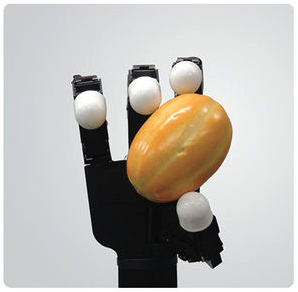
\includegraphics[width = 0.40\textwidth]{figures/01_intro/allegro_hand_and_melon.png}
\caption{The Allegro Hand and an oriental melon \cite{allegrohand}.}
\label{fig:intro:allegro_hand_and_melon}
% \vskip -0.25 true in
\end{figure}


\section{Related Work}
In Section \ref{sec:intro:box_ball_system}, we formulated a simple pushing task \eqref{eq:intro:simple_task_objective} as an optimal control problem \cite[\textsection 10]{underactuated}, and identified the non-smoothness in contact dynamics constraints as a key source of trouble in solving the problem. We have also illustrated the two major categories of model-based solutions towards the non-smoothness and their drawbacks: (\textbf{i}) nonlinear optimization using smoothed gradients of contact dynamics, which frequently get stuck in local minima, and (\textbf{ii}) considering contact mode transitions explicitly, which scales poorly due to the exponential explosion of the number of modes. 

In this subsection, after a brief review of how contacts are modeled numerically and how such modeling leads to non-smoothness, we will give a more detailed account on model-based contact-rich planning/control algorithms based on (\textbf{i}) nonlinear optimization and (\textbf{ii}) sequencing contact mode transitions. We will also discuss what model-based methods can learn from the success of applying RL to contact-rich manipulation, which has created the most impressive contact-rich manipulation demos (so far) on robotic hardware.


\subsection{Modeling Contact with Complementarity Constraints} 
\label{sec:intro:complementarity_constraints}
For a pair of rigid bodies, the contact force between them and the distance between them need to satisfy some intuitive constraints: (\textbf{i}) the contact force cannot push the bodies apart, (\textbf{ii}) the distance between the two bodies need to be non-negative, and (\textbf{iii}) non-zero contact force only exists when the two bodies are touching. 

Complementarity constraints are commonly used to mathematically represent the constraints above. In addition, the Coulomb friction law which governs the magnitude of friction forces, and the maximum dissipation principle which governs the direction of friction force during sliding, can also be represented with additional complementarity constraints \cite{stewart2000rigid, anitescu1997formulating}.

From a numerical optimization perspective, complementarity constraints are challenging to handle as they have no interior and violate constraint qualifications which are needed by gradient-based methods to converge \cite[\textsection 11]{biegler2010nonlinear}. As a result, in contact dynamics simulation, specialized algorithms such as pivoting methods or projected Gauss-Seidel \cite{SiggraphContact22} have been developed to efficiently handle the non-smoothness introduced by complementarity constraints. Instead of following the gradient of non-smooth constraints, these algorithms conduct a discrete search over which sides of the complementarity constraints are active: they start with a guess of the active sides and iteratively improves the guess until an iteration limit is reached, much like how the simplex algorithm searches for the optimal active set. Such algorithms are ideal if real-timeness is more important than physical accuracy, such as in video games: the algorithm can be terminated prematurely without satisfying all constraints. 

In contrast, contact-rich planning has different priorities: satisfaction of physics constraints is essential; and the planner has to look ahead more than one step (usually tens or even hundreds of steps) at a time. Therefore, a different set of techniques for handling complementarity constraints in the context of planning have been developed, and will be detailed in the next two sub-sections.

\subsection{Nonlinear Optimization}
\label{sec:intro:nonlinear_optimization}
An optimal control problem with contact dynamics constraints can be solved as a generic nonlinear program \cite{bertsekas1997nonlinear}. A typical gradient-based solution algorithm starts with an initial guess of the optimal trajectory, and iterates between (\textbf{i}) linearizing the cost and dynamics constraints around the current trajectory, (\textbf{ii}) updating the current trajectory in a direction that locally minimizes the cost \cite{gill2005snopt, todorov2005generalized}. 

As a consequence of the non-smoothness of contact dynamics, its linearization constructed from its gradient is no longer a good local approximation. Optimizing the cost locally with a bad understanding of the constraint landscape will lead to poor convergence behavior. 

Smoothing of contact constraints, therefore, has become an essential ingredient for good convergence when solving contact-rich planning problems. There are different ways in which smoothing can be introduced. Posa \textit{et al.}  and Manchester \textit{et al.} include the complementarity constraints directly as constraints of the optimal control problem. The complementarity constraints are relaxed to have non-empty interior \cite{posa2014direct, manchester2020variational}, thereby satisfying constraint qualifications \cite[\textsection 12]{nocedal1999numerical}. Tassa \textit{et al.} solve the optimal control problem with iterative LQR (iLQR), and imposes the dynamics constraints using rollouts \cite{tassa2012synthesis}. Their linearization of the dynamics is smoothed by regularizing the contact forces \cite{todorov2012mujoco}. Lastly, by penalizing constraint violation in the cost, Mordatch \textit{et al.} smooths contact constraints by not always strictly enforcing them and their associated non-smoothness \cite{mordatch2012contact}. Importantly, smoothing introduces some form of aphysical behavior into contact dynamics (such as the ``force-at-a-distance'' effect in Posa's relaxation \cite{posa2014direct} and MuJoCo \cite{kolbert2016experimental}), and therefore needs to be iteratively decreased in order to respect the true dynamics constraint when the solution algorithm converges.

% My assessment: they scale well but get stuck in local minima.
By ``blending'' adjacent contact modes (e.g. Fig. \ref{fig:intro:1d_box_ball}c-d), smoothing extends the region where linearization is valid, thereby improving the performance of nonlinear optimization algorithms that rely heavily on linearization of dynamics constraints. With the help of smoothing, nonlinear optimization can find trajectories for complex systems such as humanoids on monkey bars \cite{dai2014whole}. However, nonlinear optimization frequently gets stuck in local minima due to the inherent non-convexity of many contact-rich planning problems, and thus requires non-trivial initial guesses.

\subsection{Contact Mode Transitions}
Another approach to handle the non-smoothness in contact dynamics is to ``chop up'' the dynamics into smooth pieces (contact modes). The ``chopping'' makes the dynamics within modes relatively straightforward, and shifts the difficulty of the planning problem to the transitions among modes. 

Mixed-Integer Programming (MIP) \cite{bertsimas1997introduction} naturally transcribes the smooth dynamics within modes and the discrete transitions between modes using continuous and integer variables, respectively \cite{marcucci2019mixed}. For simple systems (e.g. planar linear humanoid between walls \cite{marcucci2017approximate}), it is possible to discretize the entire state space and ask MIP solvers for a \emph{globally optimal} plan. Global MIP formulations of contact-rich planning problems have very non-convex optimization landscapes, making them difficult for nonlinear-optimization-based solvers \cite{marcucci2019mixed}. 

Solving MIPs can be time-consuming and often too slow for using the planner at real-time rates as a Model-Predictive Controller (MPC). As a result, various techniques have been developed to accelerate solving MIPs in the context of contact-rich planning. Marcucci \textit{et al.} warm-start new MIPs using optimal solutions of similar problems \cite{marcucci2020warm}. Deits \textit{et al.} learned value functions for a humanoid push-recovery task, making MIPs smaller by reducing the planning horizon \cite{deits2019lvis}. Aydinoglu and Posa developed a specialized MIP solver which is based on the alternating direction method of multipliers (ADMM) and can solve small contact-rich planning problems at real-time rates \cite{aydinoglu2022real}. 

Despite these efforts to improve solver efficiency, discretizing the entire state space for even moderately large systems (e.g. pushing a box in a plane) will lead to too many contact modes for exiting methods find a solution within a reasonable amount of time (e.g. a couple of minutes). As a result, global optimality is usually given up in exchange for keeping the size of the planning problem manageable. For instance, considering only contact modes around a nominal trajectory instead of the entire state space can effectively reduce problem size \cite{hogan2020feedback, aceituno2020global}. However, by restricting the planner to search around a nominal trajectory, the ability to globally search the state space, a key feature to escape the local minima which plague methods based on nonlinear optimization, is lost. 

Is it possible to retain the ability of global search without incurring the cost of global mode enumeration? If we are willing to give up on global optimality, sampling contact modes, instead of enumerating them, is a good solution. Similar to classical Sampling-Based Motion Planning (SBMP) methods in the configuration space \cite{lavalle2006planning}, SBMP through contact builds a graph in the state space. From a node in the graph and its corresponding subgoal, the graph can be grown by randomly picking a contact mode and moving towards a subgoal as much as possible without causing a mode switch \cite{cheng2021contact, wu2020r3t}. 

SBMP with sampled mode transitions (e.g. \cite{cheng2021contact}) can handle moderately complex systems such as 3D peg-hole insertion with point fingers. It has the best scalability among all planning methods that consider mode transitions. However, the number of contact modes in more complex tasks, such as dexterous in-hand manipulation, will stagnate the search even if mode transitions are sampled instead of enumerated. This suggests that contact-rich manipulation planning may need a method that is fundamentally different from searching through mode switches.

Recently, Marcucci \textit{et al.} has developed graph of convex sets (GCS), a novel MIP formulation for optimal control problems that offers tight convex relaxations to the original MIPs \cite{marcucci2021shortest}. Similar to other MIP formulations, GCS does not scale well if the convex sets it searches through are derived from mode enumeration. However, with an appropriate decomposition of the state space that does not directly rely on contact modes, GCS could efficiently search through contact dynamics globally without giving up optimality.


\subsection{Reinforcement Learning}
Recent advances in deep RL have created impressive and convincing dexterous manipulation demos where a humanoid robotic hand in-hand re-orients a cube \cite{andrychowicz2020learning, handa2022dextreme}. A combination of domain randomization \cite{tobin2017domain} and Proximal Policy Optimization (PPO) \cite{schulman2017ppo}, the algorithm for training the policy is conceptually straightforward. Yet the complexity demonstrated in the learned policies far exceed the capabilities of the best model-based contact-rich planning methods. 

Although training an RL policy requires heavy offline computation, and the learned policy often lacks interpretability and the ability to generalize to new tasks, it is undeniable that RL has solved challenging problems with which model-based methods have struggled. Understanding the reasons behind RL's success from a model-based perspective will help us improve the performance of model-based methods. 

Recent works have attributed the success of RL to its stochastic nature, where the contact modes are abstracted by a process of sampling and averaging \cite{bundledgradients, pang2022global}. This process, termed ``randomized smoothing'', has a similar smoothing effect on contact dynamics as the various model-based smoothing schemes introduced in Sec. \ref{sec:intro:nonlinear_optimization}. Another key factor behind the empirical success of RL could lie in its goal of performing global optimization \cite{pang2022global}, which nonlinear optimization fails to do, and methods based on mode transitions can do only at limited scale.

This hints at a possible strategy of enhancing model-based contact-rich planning methods: if we could combine model-based smoothing with an efficient global search scheme, we might be able to achieve RL-level performance without incurring RL-level computational cost.


\section{Contributions and Thesis Structure}
Smoothing and global search are both essential to the success of contact-rich planning, but as far as we know, no existing method does both. This thesis proposes a contact-rich planning algorithm that searches globally under the guidance of a smoothed contact model. The proposed method can, within 1-minute of wall-clock time on a regular desktop computer, generate contact-rich plans for complex robotic systems such as dexterous hands.

At the heart of the model-based planning approach we took lies the question: what is the \emph{right} model for contact-rich manipulation? In Chapter \ref{chapter:quasi_static_dynamics}, we present a novel formulation of rigid-body contact dynamics that is quasi-static, convex, differentiable and amenable to smoothing, all of which are features chosen to improve the efficiency of the planner.

In Chapter \ref{chapter:contact_rich_planning}, we present the global contact-rich planner that utilizes the proposed quasi-static contact model and combines SBMP with trajectory optimization. Efficient global exploration is carried out with a kino-dynamic sampling-based motion planner that searches with large step sizes near the contact manifold. By abstracting contact modes away with a smoothed version of the contact dynamics, the sampling-based planner can effectively explore the state space without suffering from the exponential explosion of contact modes. Once a coarse path is found by the sampling-based planner, the path is refined by a trajectory optimizer with finer step sizes to improve its quality and physical accuracy. 

The challenges facing contact-rich manipulation extend far beyond planning. Once a plan is generated, interaction forces between the robot and the objects need to be sensed and estimated. The estimated forces, together with other estimated states, are then fed to a stabilizing controller that is aware of making and breaking contacts. 
Therefore, this thesis also explores (\textbf{i}) external contact force estimation from joint torque measurements (Chapter \ref{chapter:force_from_torque}), and (\textbf{ii}) reconciling tracking trajectory and bounding contact forces using a inverse-dynamics controller in the simple case of interacting with a static environment (Chapter \ref{chapter:quasi_static_control}). Interestingly, the methods in both Chapter \ref{chapter:force_from_torque} and \ref{chapter:quasi_static_control} benefit from the simplifying quasi-static assumption, highlighting the utility of quasi-static dynamics in various components of the robotic manipulation pipeline. 



